\documentclass[tikz]{standalone}
\usepackage{amsmath,amssymb}
\usepackage{pgfplots,multicol}

\pgfplotsset{compat=1.13}
\usepgfplotslibrary{fillbetween}

\begin{document}


 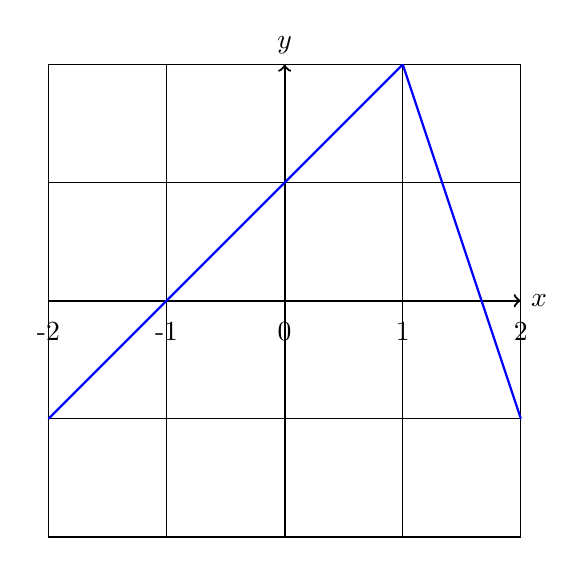
\begin{tikzpicture}[scale=1.5,	declare function={ f(\x) =abs(sin(\x*90)); g(\x) =3*abs(sin(\x*90)); 
                 }]

    \draw[->,thick] (-2,0) -- (2,0) node[right] {$x$};
    \draw[->,thick] (0,-2) -- (0,2) node[above] {$y$};
    \draw[step=1.0,black,thin] (-2,-2) grid (2,2);
\foreach \x in {-2,-1,0,1,2} \draw (\x,0.1) -- (\x, -0.1) node[below] {\x};

\draw[-,color=blue,smooth,domain=-2:1,thick] plot(\x,{\x+1});
\draw[-,color=blue,smooth,domain=1:2,thick] plot(\x,{-3*\x+5});

\end{tikzpicture}

	
\end{document}
